
\documentclass{article}

\title{The Physics of Energy Transfer}
\author{Henok Abatihun Birhane \\
	henokapat@gmail.com \\
	henokabat@icloud.com \\
	@henokapat (x.com)}
\date{\today}
\setlength{\parskip}{.5em}
\usepackage{graphicx}
\usepackage{tcolorbox}
\usepackage{float}
\usepackage{url}
\usepackage{cite}
\usepackage{amsmath}

\begin{document}

    \maketitle


    \begin{abstract}
        Isaac Newton defined the laws of motion and gravity~\cite{newton1687principia}, which were later expanded upon by Albert Einstein through his deeper understanding of time and gravity~\cite{einstein1905electrodynamics} ~\cite{einstein1916foundation}.
         However, Einstein himself was not fully satisfied with his theory.
         He believed that the theory of relativity offered only a limited perspective, aimed at improving measurement and relative observation, and that it still left certain aspects of time and gravity unexplained.
         This paper discuss narrower view of the cause for time, inertia and gravity based on newton, Einstein and multiple experiment results.
         The question \('\)of why' for time, inertia and gravity will be discussed
    \end{abstract}

    \newpage
    \section{Distance}\label{sec:distance}
    Distance is a fundamental measurement of space, commonly expressed in meters.
    However, when measuring distance in a moving environment, such as a planet or a spaceship, the measurement becomes more complex.
    Human distance measurement does not consider the motion of planets, spacecraft, and other celestial bodies that are constantly traveling in space.

    For instance, if we measure the distance traveled by an object inside a spaceship, the reading only reflect its movement within the spacecraft.
    However, if the spaceship itself is moving through space at high velocity, the object’s true distance traveled would be much greater.
    Similarly, measuring distance on Earth does not take into account the fact that Earth itself is orbiting the Sun and moving through the galaxy.

    Distance has to reflect actual distance in space to calculate speed of objects, light, and other energy packets in space.

    \section{Energy}\label{sec:energy}
    Energy is multiplication of two fundamental elements: mass (matter) and the velocity at which that matter moves.
    To increase energy, either the amount of matter or its speed must increase.
    For an object to remain at rest or move at a constant velocity, the total energy input and output in all directions must sum to zero~\cite{newton1687principia}.

    For an object to remain at rest or move at a constant velocity, the total energy input and output must balance, maintaining a net energy change of zero.
    If an object interacts with two identical masses approaching from opposite directions at the same speed, the energy exchange remains balanced, resulting in no change in motion.
    Likewise, when an object expels equal amounts of mass in opposite directions at the same velocity, the system conserves energy and momentum, ensuring the object does not change in motion~\cite{newton1687principia}.

    For an object to remain at rest or move at a constant velocity while releasing and receiving energy in the same direction then incoming and outgoing are canceling out.
    Imagine a mass attempting to escape from a system, but held in place by a pulling(binding) energy.
    Just before it can break free, another identical mass approaches from the escape direction and collides with it, stopping the scape.
    The original mass experiences no net change in motion and both the incoming and outgoing masses are identical and interact simultaneously, the two must have had equal speed.
    This implies that their motion effectively cancels out.


    \begin{tcolorbox}[colback=white, colframe=black, boxrule=1mm, arc=4mm, auto outer arc]
        Law 1: If an object experiences no change in motion when two identical masses approach from opposite directions and attach to it, then the two approaching objects had been moving at the same speed in space but opposite directions.
    \end{tcolorbox}

    \begin{tcolorbox}[colback=white, colframe=black, boxrule=1mm, arc=4mm, auto outer arc]
        Law 2: If an object experiences no change in motion when releasing two identical masses in opposite directions at the same moment, then the two released objects must have the same speed in space but opposite directions.
    \end{tcolorbox}

    \begin{tcolorbox}[colback=white, colframe=black, boxrule=1mm, arc=4mm, auto outer arc]
        Law 3: If an object experiences no change in motion when release and receive  identical masses at the same moment, then the two received/released objects must have the same speed in space  at similar or opposite directions.
    \end{tcolorbox}


    \section{Photon}\label{sec:photon}
    Photon can push and put a pressure on object which is the characteristic of energy that proofs photon are a valid very small energy packet~\cite{einstein1905electrodynamics}.

    When energy is applied to two objects of vastly different sizes, causing them to move in opposite directions, the smaller object will accelerate much faster than the larger one.
    In contrast, the larger object will exhibit only slight movement due to its greater mass.
    Photons are the fastest known energy packets in the universe.
    Their fastest speed suggests that photons are the smallest possible units of energy packet human able to observe.
    Furthermore, the fact that photons always travel at a constant speed in space indicates that a fixed amount of energy is sufficient to propel them at that speed~\cite{einstein1905electrodynamics}.

    Photons and photon-like energy packets are emitted from objects in all directions, such as the Sun, Earth, and Voyager 1.
    These objects not only release photons into outer space but also exchange these energy packets internally—between their atoms, electrons, nuclei and between other possible combinations.
    Despite the continuous emission and absorption of these energy packets, the speed of these objects remains unaffected, as the seemingly random direction of photon release cancels out any overall motion effect on the source, in accordance with Law-1.
    The object’s random release/absorption direction of photon, constant mass of photon, and constant speed of photon  ensure that photons do not alter object’s motion, as stated by Law-1, Law-2 and Law-3.

    \section{Time}\label{sec:time}
    This section discusses the validation of the following theory

    \begin{tcolorbox}[colback=white, colframe=black, boxrule=1mm, arc=4mm, auto outer arc]
        Theory 1: A photon approaches or moves away from an observer at a speed equal to C ± V.
        \begin{itemize}
            \item Where
            \begin{itemize}
                \item C = speed of the photon in space
                \item V = speed of observer parallel to photon movement direction
            \end{itemize}
        \end{itemize}
    \end{tcolorbox}

    Time is the measurement of energy change.
    Energy change occurs when an object either transfers or receives a portion of its energy.
    Energy transfer happen as photon and photon-like energy packets between objects.
    Time also can be defined as the measurement of energy transfer rate between objects.
    The higher transfer rate, the higher time.
    Experiments\cite{bailey1977} indicated that for specific transfer rate (time) while object is moving at given speed, if the object speed increased time will slow down.
    Let look into how that is the case:

    Assumptions:
    \begin{itemize}
        \item Objects A and B are separated by a distance D in space
        \item Object B reflects photons.
        \item When Object A emits a photon, and the photon is reflected by Object B and returns to A, a time change occurs over the span of one second.
    \end{itemize}

    If Object A and B is at rest then 1 second represents 2D photon distance coverage in space.

    Lets calculate photon distance coverage by assuming A nd B are traveling at 0.5C in space as shown on bellow diagram.

    \begin{itemize}
        \item When photon arrive at B, it covered 2D distance.
        \item When photon return back to A, it covered additional 2D/3
        \item Total distance coverage for photon is 2D + 2D/3 = 8D/3
        \item 1 second represent 8D/3 photon distance coverage in space.
    \end{itemize}

    \begin{figure}[H]
        \centering
        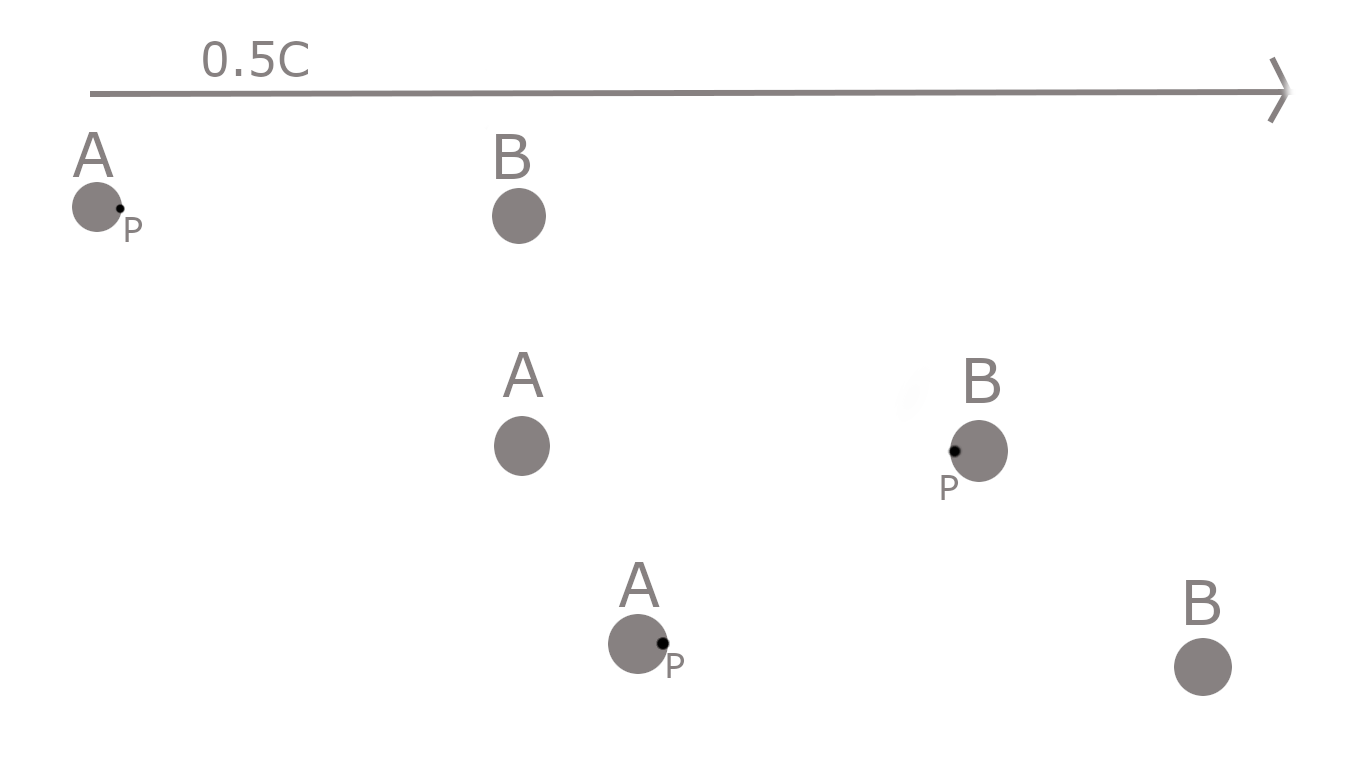
\includegraphics[width=0.8\textwidth]{images/horizontal-time-relativity}
        \caption{Horizontal time relativity}
        \label{fig:time relativity}
    \end{figure}

    If we call t as time while A, B is at rest and t' when A and B moves at 0.5C, the comparison will be as follows:

    \begin{gather*}
        t(2D) = t'\left(\frac{8D}{3}\right)\\
        t = \frac{4}{3} t'\\
        t \approx 1.333 t'\\
    \end{gather*}


    We can calculate general formula for horizontal time relativity.

    Photon distance coverage for rest A and B objects can be defined:

    t = 2D

    D = t/2

    When A and B moves at the same speed in the same direction, AB and BA photon distance coverage will re-adjust from t'/2 as follows:
    \begin{itemize}
        \item When photon arrive at B, it covered C(t'/2)/(C-V) distance or (2D).
        \item When photon return back to A, it covered additional C(t'/2)/(C+V) distance or (2D/3)
        \item Total distance coverage for photon is C(t'/2)/(C-V)+ C(t'/2)/(C+V)

        \begin{gather*}
            t = \frac{C \left( \frac{t'}{2} \right)}{C - V} + \frac{C \left( \frac{t'}{2} \right)}{C + V}\\
            t = \frac{t'}{1 - \frac{V^2}{C^2}}\\
        \end{gather*}

        where:
        \begin{itemize}
            \item \( t \) is the horizontal rest time,
            \item \( t' \) is the horizontal moving time,
            \item \( V \) is the velocity of the moving object with time t,
            \item \( C \) is the speed of light with time t.
        \end{itemize}

    \end{itemize}

    The time experienced by an object depends on the exchange of photons in all directions.
    These exchanges are influenced by the object’s motion, with the observed time being an average of both horizontal and vertical photon interactions respective to its direction of travel.

    When a photon travels vertically relative to an object’s motion, it may escape into outer space if the object’s movement shifts the destination far enough for the photon to miss its target.
    In reality, time is governed by the exchange of photons and photon-like energy packets between atoms, electrons, nuclei, and other possible interactions.
    These interactions occur over extremely short distances, reducing the probability of escape to an insignificant level.
    we can consider photon hit C and come back to A. Vertical motion is zero and the distance between A and C will stay the same while photon travel from A to C. Photon will travel 2D distance while traveling A to C and back to A\@.


    \begin{figure}[H]
        \centering
        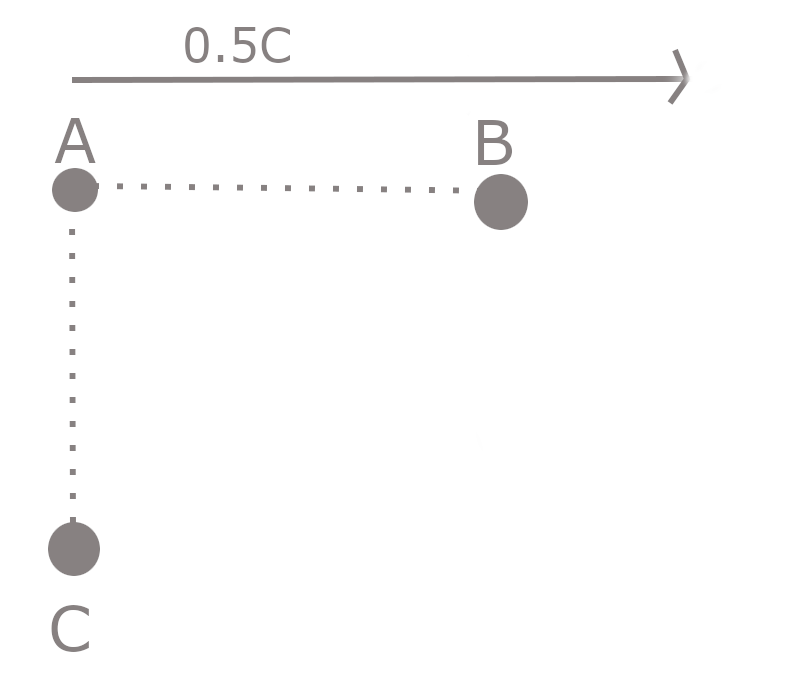
\includegraphics[width=0.8\textwidth]{images/avarage-time-relativity}
        \caption{Average time relativity}
        \label{fig:avarage time relativity}
    \end{figure}

    The vertical and horizontal time differences to the moving object can be calculated as previously demonstrated.
    Now, using these vertical and horizontal values, let’s determine the average time difference.
    The time difference increases at constant rate from vertical to horizontal.
    The average is middle time difference of horizontal and vertical.

    \begin{figure}[h!]
        \centering
        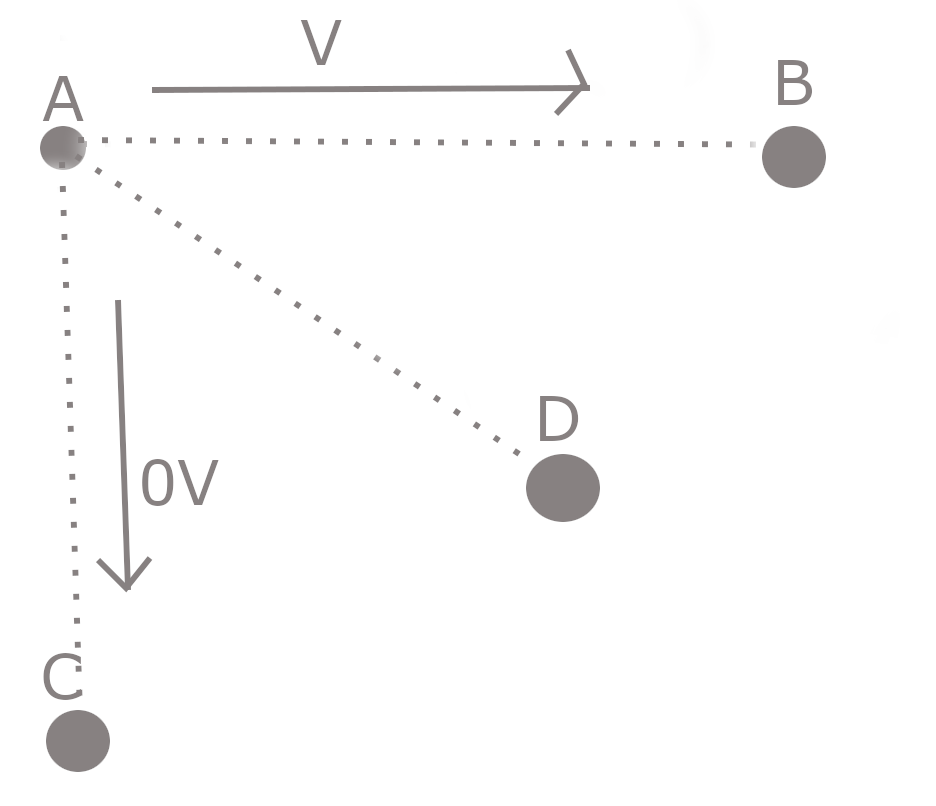
\includegraphics[width=0.8\textwidth]{images/avarage-time-velocity}
        \caption{Average time}
        \label{fig:avarage time velocity}
    \end{figure}

    \begin{itemize}
        \item Vertical, A to C back to A , time calculated as:
        \[
            t = {t'}{1}
        \]
        \item Average, A to D back to A, time be calculated as:

        \[
            t = {t'}{x}
        \]
        x is unknown value

        \item Horizontal, A to B back to A, time be calculated as:

        \[
            t = {t'}{x}{x}
        \]

        Using horizontal time difference formula formulated above:

        \begin{gather*}
            t = \frac{t'}{1 - \frac{V^2}{C^2}}\\
            {t'}{x}{x} = \frac{t'}{1 - \frac{V^2}{C^2}}\\
            {x} = \frac{1}{\sqrt{1 - \frac{v^2}{c^2}}}\\
        \end{gather*}
        When we insert  value to the average time difference:
        \begin{tcolorbox}
            \begin{gather*}
                t = {t'}{x}\\
                t = \frac{t'}{\sqrt{1 - \frac{v^2}{c^2}}}\\
            \end{gather*}

            \begin{itemize}
                \item \( t \) is the average rest time,
                \item \( t' \) is the average moving time,
            \end{itemize}average

        \end{tcolorbox}
    \end{itemize}

    This formula is exactly equivalent to the Lorentz time dilation expression.
    It derived above under the assumptions of Theory 1, thereby serving as a proof of Theory 1.

    The probability of photon need medium to travel in space is very low as a planet does not need medium to travel though space.
    Photon is small version of planet or asteroid.
    if large objects move without medium in space, small energy packets like photon will not have obstacle to travel in space.
    Their smallness will give them the advantage to travel in great speed with small energy push.

    An experiment~\cite{michelson1879velocity} confirms that light travels at a constant speed with time t and t', where t corresponds to 2AB and t' to 2A'B'. A' and B' are points on moving object and the photon exchange between A' and B' can be shown as follows.

    Bulb is A' and mirror is B'


    \begin{figure}[H]
        \centering
        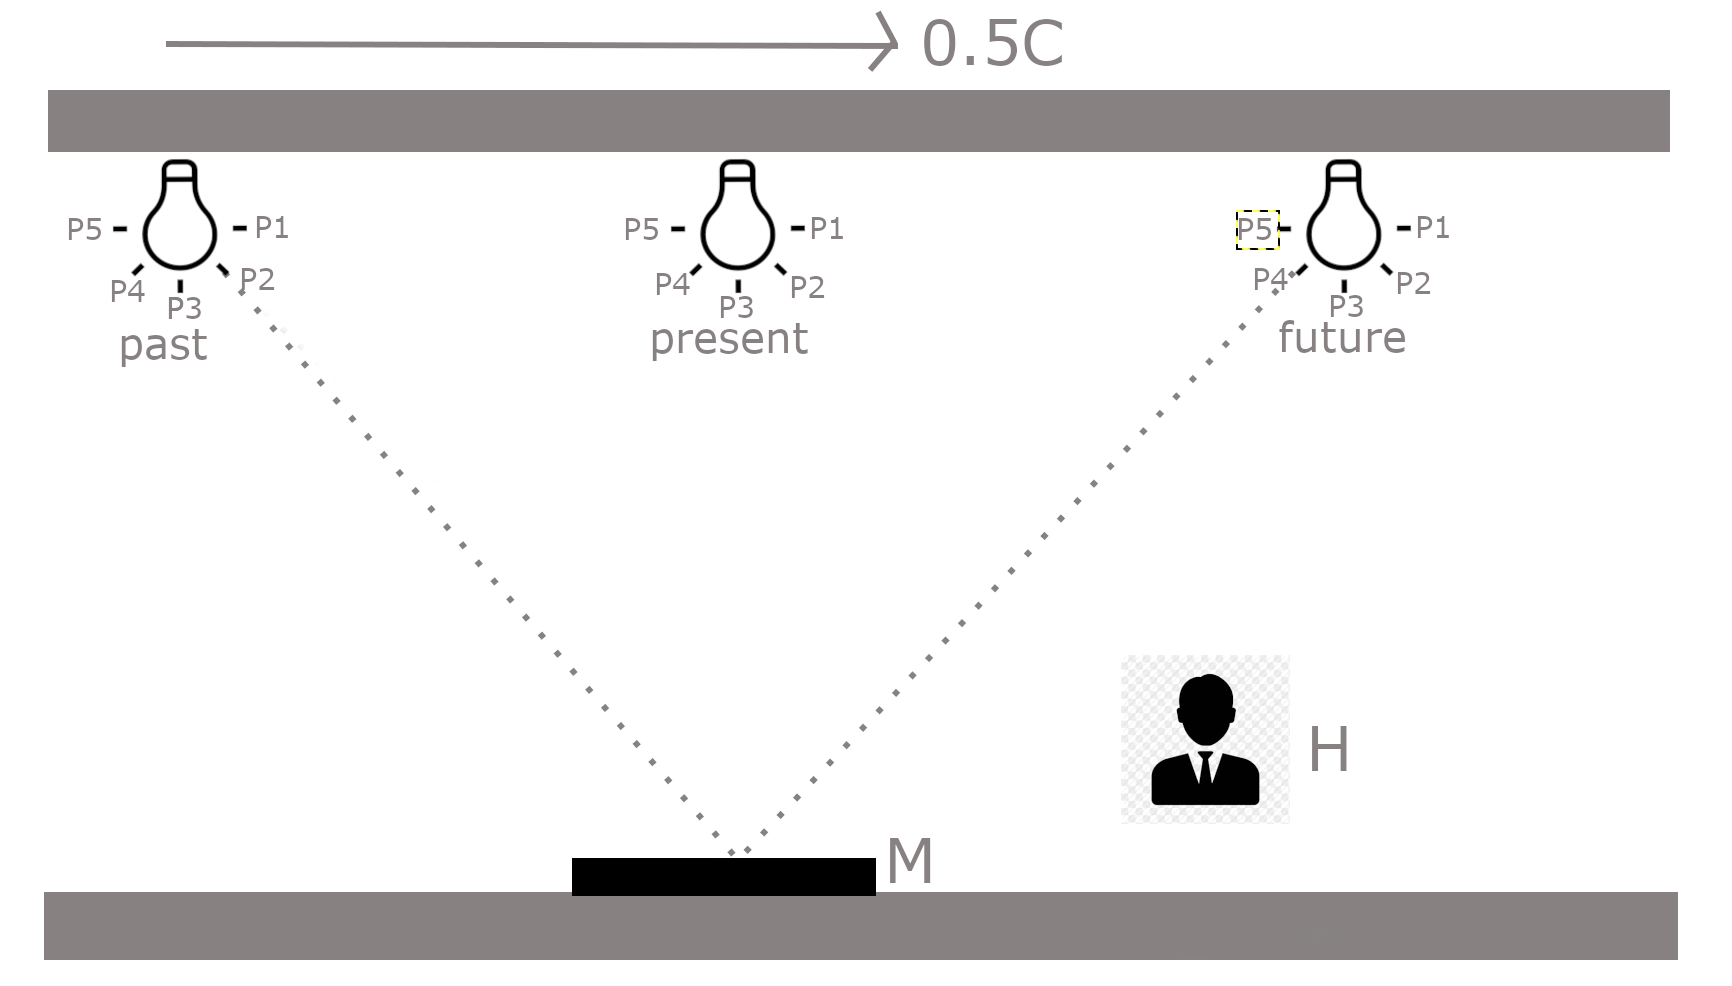
\includegraphics[width=0.8\textwidth]{images/photon_path_and_distance}
        \caption{Photon path and distance mesurment}
        \label{fig:photon_path_and_distance}
    \end{figure}

    Mister H is aboard a ship traveling at 0.5 times the speed of light.
    H is trying to measure the distance from bulb to the mirror using light.
    When the measurement begins, the photon emitted from the bulb toward P2 will strike the mirror and return to the bulb in the direction of P4. Mister H has neither the knowledge nor the awareness that the ship is traveling at half the speed of light He will have also difficulty detecting the photon emitted in the direction of P2, rather than P3, is the one that strikes the mirror.
    If Mister H uses a laser instead of a bulb, he will still adjust the laser in the direction of P2 to hit the mirror, mistakenly believing he is aiming at P3 direction.
    Finally, mister H think the photon traveling between the bulb and mirror in straight line as P3-Mirror-P3 but in reality photon is traveling P2-Mirror-P4 in diagonal straight line.
    The photon path P2-Mirror-P4 follows the same trajectory as the average photon path A-D-A (figure~\ref{fig:avarage time velocity}). The distance covered by the photon and the average time measurement(t’) are both diagonal, demonstrating that both increase at the same rate.
    Same rate increase confirms that the speed of light is constant for  2AB with t and 2A'B' with t'.

    The speed of a photon with paths 2AB and 2A’B’ has been tested using Michelson’s experiment~\cite{michelson1879velocity} and modern laser interferometry~\cite{evans1972measurement}.
    Modern laser interferometry tries to examines light traveling along different paths but covering the same distance, ensuring that both beams reach their destination simultaneously.
    The experiment assumes photon travel straight line into parallel mirror but  as we discuss above the photon will move in diagonal path on moving planet earth.

    \begin{figure}[H]
        \centering
        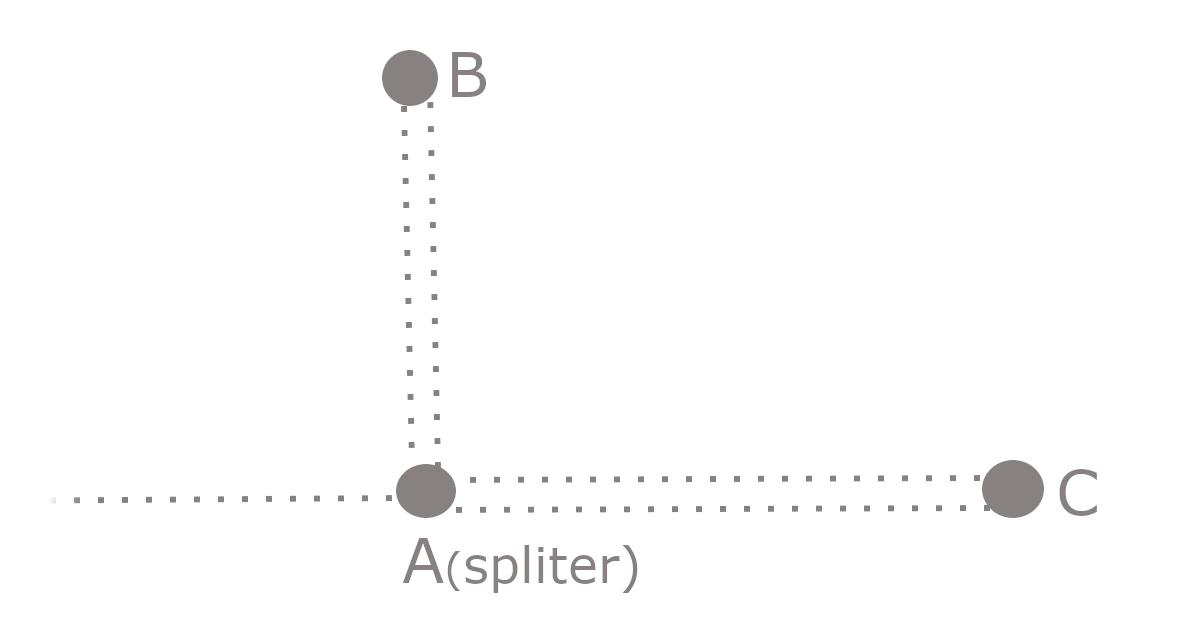
\includegraphics[width=0.8\textwidth]{images/interferometry_expected_photon_phath}
        \caption{Expected path of photon in interferometer}
        \label{fig:interferometry_expected_photon_phath}
    \end{figure}



    \begin{figure}[H]
        \centering
        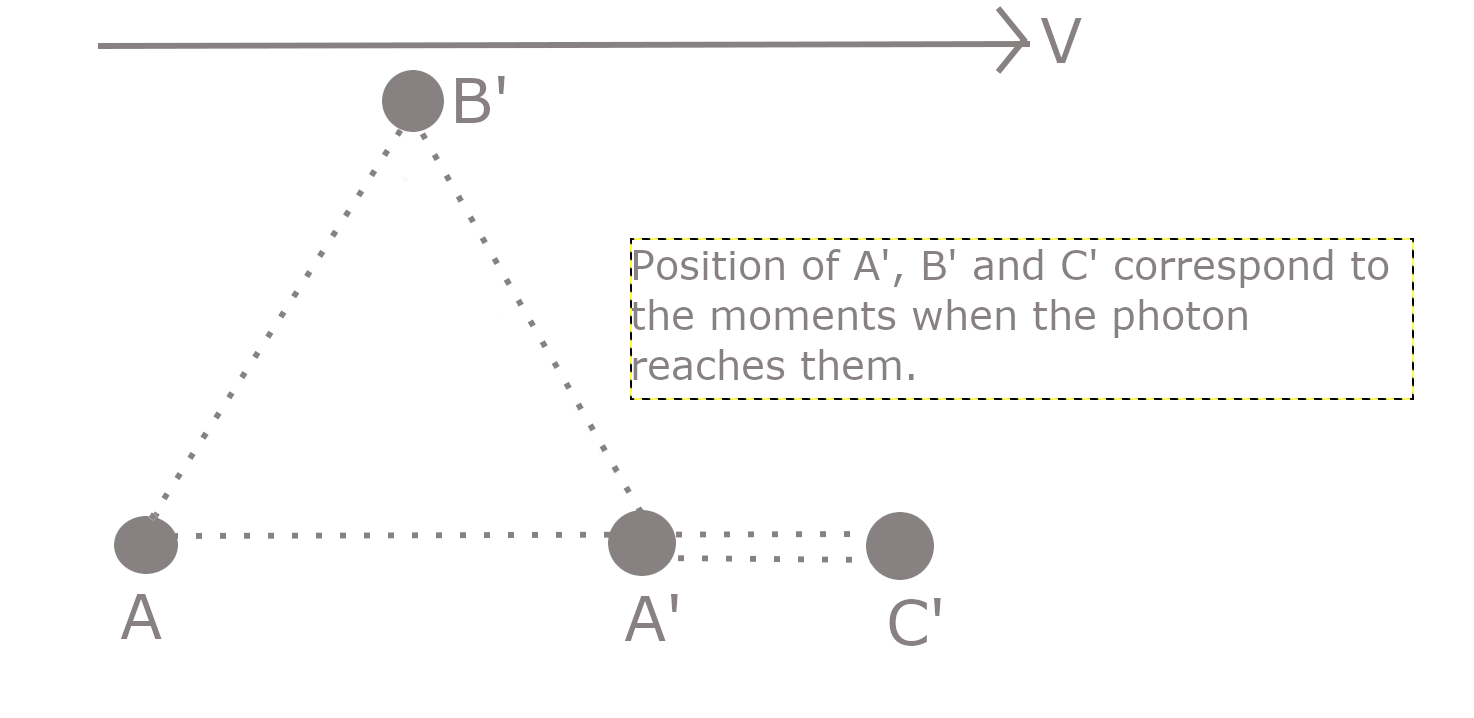
\includegraphics[width=0.8\textwidth]{images/interferometry_actual_photon_phath}
        \caption{Actual path of photon in interferometer}
        \label{fig:interferometry_actual_photon_phath}
    \end{figure}

    Earth is moving at speed V in the direction of A-C. When the interferometer is set up, the splitter is adjusted to reflect the photon in a direction that ensures it reaches B, expected straight, actual diagonal straight.

    \begin{itemize}
        \item Path one = AB'A'
        \item Path two = AC'A'
    \end{itemize}

    Calculating AB'A' with pythagoras theorem exactly equals with AC'A'. Photon covers in both path the same distance resulting interface to happen in the experiment.


    \section{Ineartia}\label{sec:ineartia}
    An object can either remain at rest or move at a constant speed through space~\cite{newton1687principia}, demonstrating that space itself does not interfere, resist, or impose obstacles to slow down or accelerate the object’s motion.
    If space does not influence an object that is either at rest or moving at a constant speed, suggests that it will not oppose the object’s ability to accelerate or decelerate.

    Two objects may compete for space if they move in opposite directions with non-zero speed toward each other.
    In this scenario, collisions occur as they struggle for position, with the larger object or the one with greater speed ultimately prevailing.
    In this situation, it is understandable for A to exert force on B and vice versa, as they are both traveling to each other competing for the same space.

    When A moves toward B, A is approaching B with a nonzero speed in space, but B is not approaching A. When A collides with B, A exerts a force on B due to its velocity  towards B. Ideally, B should move easily in response to A’s force.
    However, instead of moving freely, B applies a resistance force against A. This resistance force means that after A hits B, B acquires a nonzero speed toward A.

    Zooming-in to large objects that are either at rest or moving at a constant speed reveals electrons, atoms, and other combinations exchanging photons and photon-like energy packets between them.
     When an object is at rest in space, the frequency of photon exchange between its atoms and other pairs remains the same in all directions.
     The speed of a photon or energy packet traveling from A to B in space is c.
     Both A and B emit and receive photons or energy packets at the same frequency (rate).
     Since the frequency (matter) and speed remain the same for both A and B, there is no net change in velocity for A, B, or the larger object that encompasses them, as stated by Rule 3.
      This net zero will keep the object at rest forever in space.

    When an object moves at speed V, the exchange frequency of photons or energy packets will vary in space.
    However, the speed of these photons or energy packets in space will remain c.

    \begin{figure}[H]
        \centering
        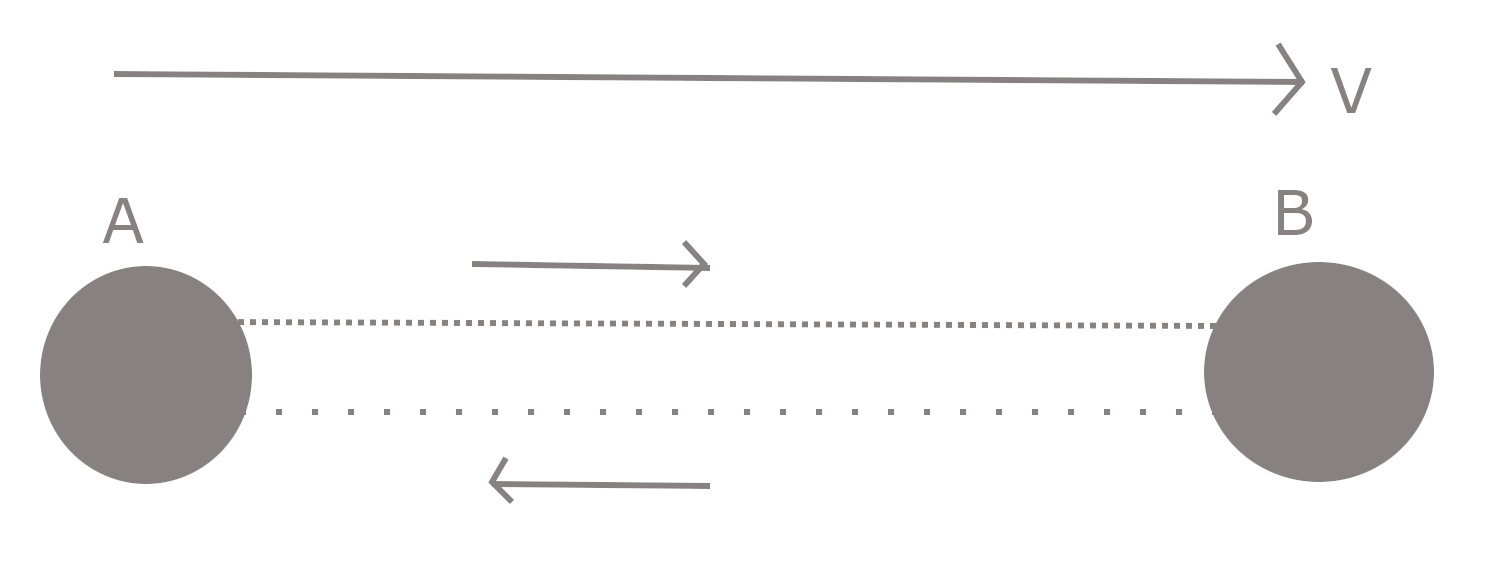
\includegraphics[width=0.8\textwidth]{images/inertia_constant_velocity}
        \caption{Exchange of photon or energy-packets at constant velocity}
        \label{fig:inertia_constant_velocity}
    \end{figure}

    A moving object keep moving in space indefinitely, which indicate there is net-zero on A and B while they're exchanging energy packets.
    Let’s take A and calculate whether the frequency of photons, along with the speed of absorption and release, satisfies Rule 3 for the object that contains A to continue its motion in space.

    \begin{itemize}
        \item Speed
        \begin{itemize}
            \item Photon/energy-packets  approaching A  at speed c + v and leaving A at speed c - v but travels at the same speed c in space, approach and leaving speed balance out to c.
            Rule-3 speed component satisfied.
        \end{itemize}
        \item Frequency(rate)
        \begin{itemize}
            \item outgoing frequency is (blue-shifted - v) and the incoming frequency is (red-shifted + v).
            \item (blue-shifted - v) = normal frequency
            \item (red-shifted + v) = normal frequency
            \item Both incoming and outgoing frequency are normal(equal) frequencies, Rule-3 mass component satisfied.
        \end{itemize}
        \item Mass and speed component satisfaction for Rule-3 leads the object that contains A, B to travel space with the same speed forever.
    \end{itemize}

    Object is at rest or at V then when it is accelerated or decelerated it will generate non-zero approach velocity in the direction of acceleration cause, called inertia.

    Let's say we accelerated Figure~\ref{fig:inertia_constant_velocity} from direction A. The acceleration push will accelerate A first and result the photon frequency from A to B be more blue shifted.
    once the increased blue shifted reach B at speed c, B will accelerate by the increased blue shifted frequency and sync with A. if the acceleration force stops and the increased blue shifted reaches B, the object that contains A and B will continue moving with the accelerated v forever.
    The resistance non-zero approach velocity in the direction of accelerator is from A.  The non-zero resistance v is generated by A before the sync with B\@.
    \begin{itemize}
        \item x will be the added velocity by the acceleration.
        \item Speed
        \begin{itemize}
            \item Photon/energy-packets  approaching A  at speed c + (v + x) and leaving A at speed c - (v + x) but still travels at the same speed c in space, approach and leaving speed balance out to c.
            Rule-3 speed component satisfied.
        \end{itemize}
        \item Frequency(rate)
        \begin{itemize}
            \item incoming frequency stays the same as original red shifted since B is not yet affected by the acceleration.
            \item outgoing frequency is (more blue-shifted - (v+x)) and the incoming frequency is (red-shifted +( v+x)).
            \item More blue-shifted - (v+x) = normal frequency
            \item red-shifted +( v+x) = normal frequency + x
            \item Outgoing is still normal frequency  but incoming frequency is increased by x which results A to approach the accelerator with non-zero v' velocity.
            Rule-3 not satisfied
            \item A is surrounded with particles other than B at different angles.
            The incoming frequency from all those will increase, moving A towards the accelerator.
            \item In-conclusion, when the right  side frequency increase because of the accelerator, left side frequency  will increase pushing against accelerator.
        \end{itemize}
        \item The above proofs that A is having v' velocity towards accelerator.
         There are millions, billions pair of AB even in small object, all of  A have v' approach towards accelerator and resulting the effect of inertia.
    \end{itemize}

    \section{Gravity}\label{sec:gravity}
    The Earth pulling the Moon, and the Sun pulling the Earth, are both examples of gravity.
    It’s unlikely that Sun has a magical rope stretching through space to keep pulling the Earth.
     One thing possible is sun hitting earth with energy-packets like photon, this is even visually visible with photon.
     photon is not the only energy-packet exchanged by sun-earth, earth-moon, object-object, atom-atom, nucleus-electron, electron-electron etc.
     Energy packets will continue to travel at c until they encounter an absorber or reflector as has been experimentally observed.
     The density of these energy packets will decrease for the increase of radius.
     Radius is the distance between source and current measurement point in space.

    \begin{figure}[H]
        \centering
        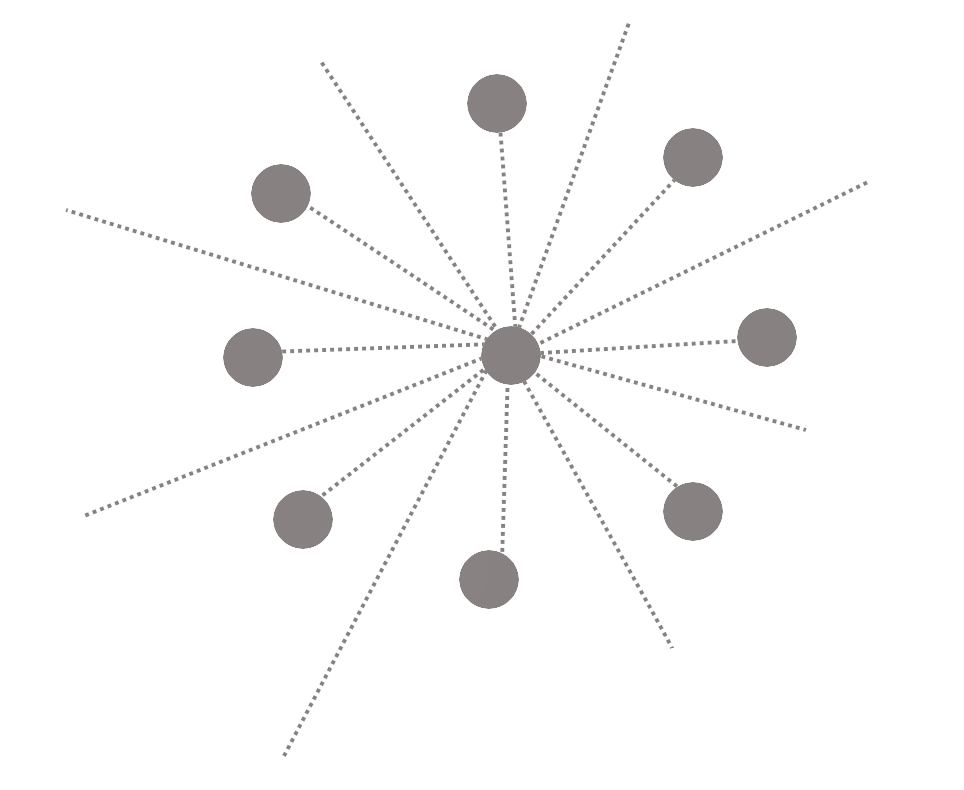
\includegraphics[width=0.8\textwidth]{images/scapping_energy_packet}
        \caption{Scaping energy packets}
        \label{fig:scaping_energy_packets}
    \end{figure}

    While discussing inertia we look into the energy package exchange between two nearby electron, atoms etc.
    Not all energy packets released from A will be captured by B. Some may escape and be absorbed by other B or lost into outer space.
    There is also a standalone, unpaired particle in space that continuously emits energy packages.

    \begin{figure}[H]
        \centering
        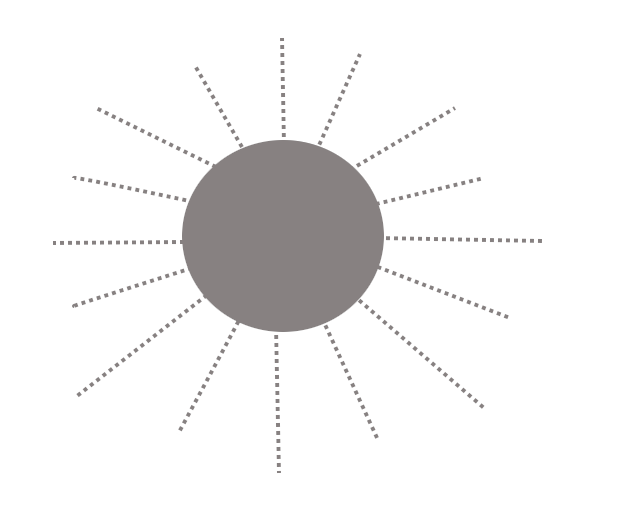
\includegraphics[width=0.8\textwidth]{images/energy-packet release}
        \caption{particle releasing energy packets}
        \label{fig:energy_packet_single_object}
    \end{figure}

    Net motion effect at A in Figure~\ref{fig:scaping_energy_packets} and~\ref{fig:energy_packet_single_object}  is zero.
    If A is at rest, it will remain at rest; if it is in motion, it will continue moving—even while releasing energy packets—because the net effect is zero according to Rule-2 and Rule-3.

    The equilibrium shown in Figure~\ref{fig:scaping_energy_packets} and~\ref{fig:energy_packet_single_object} will no longer exist when a similar object is placed nearby.
    Let’s assume there are two Figure~\ref{fig:energy_packet_single_object} objects positioned close to each other in space, with no third object present, call them A and B. The object(A) is now not only releasing energy packets in all directions, but also receiving energy packets from B. The net exchange at A in the direction of B is Xa - Xb when X is the number of energy packets.
    The density of energy packets decreases with distance from the source.
    When Xb reaches point A, it has traveled a distance r(BA), which significantly reduces the number of energy packets that reach A. The greater the distance r, the more energy packets miss object A\@.

    \begin{figure}[H]
        \centering
        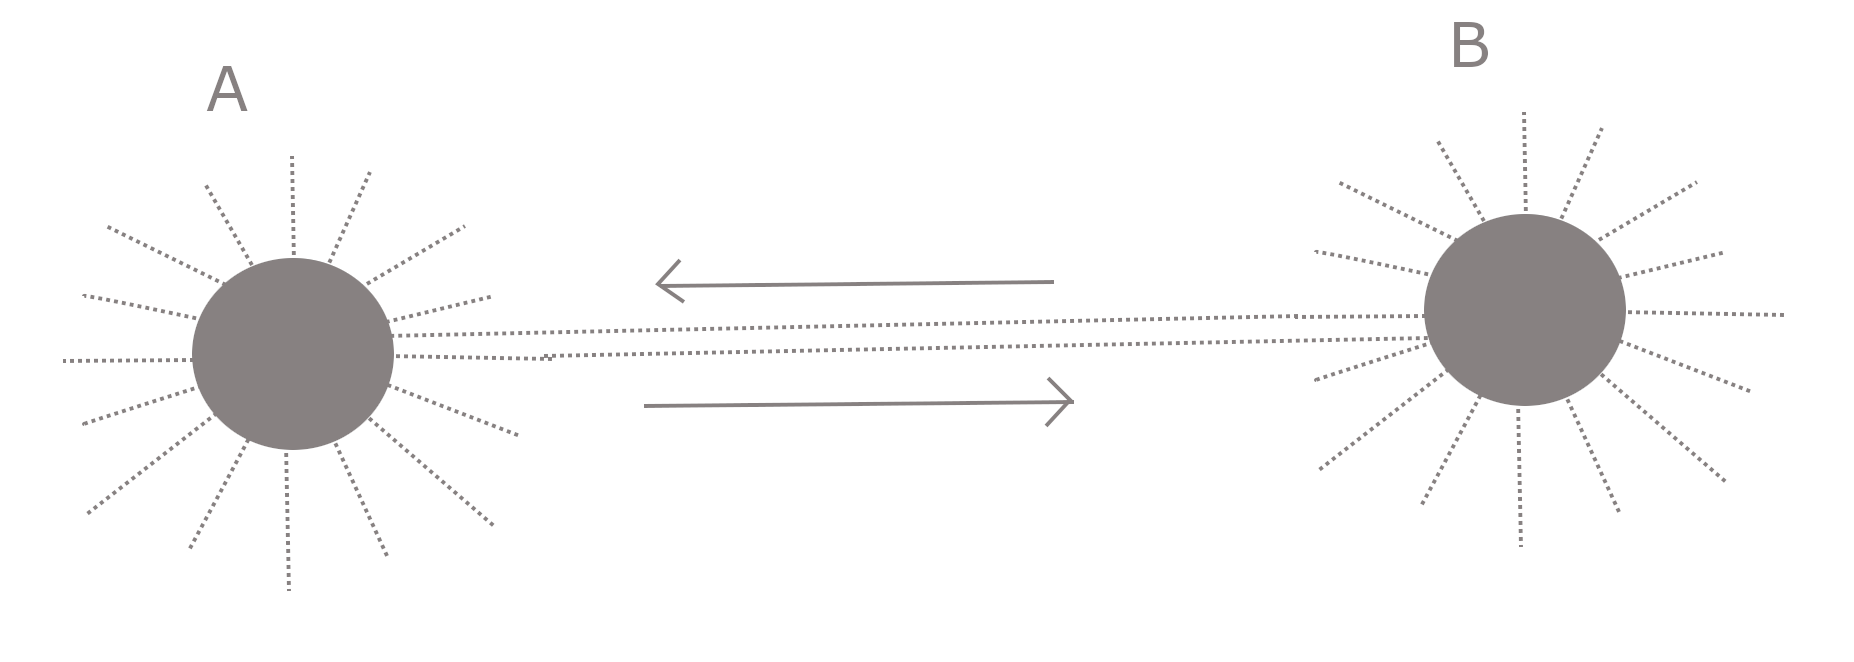
\includegraphics[width=0.8\textwidth]{images/gravity_between_two_object}
        \caption{Two object exchanging energy packet}
        \label{fig:gravity_between_two_object}
    \end{figure}

    The energy-packet release of A in the direction of B is Xa-Xb which is less than Xa of other directions.
     The equilibrium for Rule-2 is not satisfied.
     A is releasing less net energy packets in the direction of B resulting nonzero push by the released energy packets in the opposite direction towards B. A will start moving in the direction of B.  The same effect will happen to B,  and it will start moving to A. This effect called gravity.

    Two or more Figure~\ref{fig:energy_packet_single_object} moves to each other and create Figure~\ref{fig:scaping_energy_packets}.
    Collection of Figure~\ref{fig:scaping_energy_packets} will create atoms, molecules, planet, star and black hole.

    The density of Xb decreases exponentially as r increases.
    Even at short distances, Xb remains significantly lower than Xa as the result seeing the effect of gravity on medium objects like between two elephant is insignificant.
    To increase the density at a given r, increase the number of B\@.

    \begin{figure}[H]
        \centering
        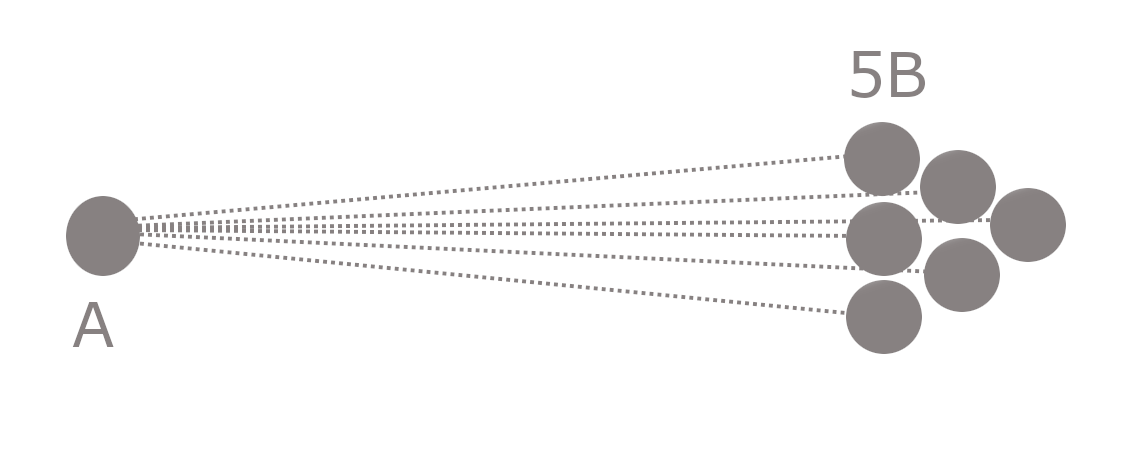
\includegraphics[width=0.8\textwidth]{images/gravity_multiple_B}
        \caption{Strength of gravity}
        \label{fig:gravity_multiple_B}
    \end{figure}

    Planet like earth has uncountable very large number of B's resulting significant density of energy packets in the surroundings r space.
    Gravity is significant  around earth.
    Still Xb from earth is very small compared to Xa for single A. Xa is the density when r = 0.
    To push A instead of pull, requires generating  $ Xb > Xa $ at $ r > 0 $.


    \section{Infinity}\label{sec:infinity}

    Time, inertia and gravity for objects like electron, atom, molecule, planet etc is the result of energy packet exchange with photon or  similar size packet.
     If we able to zoom into photons, most probably smaller energy packets been released/absorbed from photon.
     Photons is becoming Figure~\ref{fig:energy_packet_single_object} and with the collection it becomes Figure~\ref{fig:scaping_energy_packets}.
     Time, inertia and gravity repeat itself between photons.
     The gravity effect observed as light being curved around large collection of photons like planet.

    When photon is hit by this smaller energy packet it will slow down as discussed with gravity effect, but if the hit was in the direction of photon travel it will speed up.
    In conclusion photon travel with c- when it travels away from like planet and with c+ when traveling to the planet.

    If c- and c+ are equal then average will be zero and time that is caused by photon exchange for large object should be the same near gravity and space.
    Experiments~\cite{Ashby2002} showed that time slow down near gravity.
    yes, c+ and c- are not equal for photon near gravity and the net speed will be c-x, where x is above zero.

    While discussing time we disused photon distant coverage ABA. let is have the same ABA path where A bellow and B above in terms of gravity.
    Gravity originates from point A, meaning the gravitational pull (and thus the density) is stronger near A than near B. 
    This causes the photon’s journey from A to B to be stretched out more than the return trip is shortened.
    The reason is that as the photon emerges from point A, it immediately decelerates under the influence of strong gravity and continues to move under this influence until it reaches B.
    On the return trip, however, the object begins in the weaker gravity near B, so it accelerates more slowly. Although stronger acceleration occurs as it nears A, this happens near the end of the journey.
    As a result, the object spends more time moving through the weaker gravity near B and less time in the stronger gravity near A. 
    Therefore, the extra time spent during the slower part of the journey isn’t fully compensated by the time saved during the faster part.
    Consequently, the total round trip from A to B and back to A takes longer than it would in the absence of gravity even though the total distance traveled (2d, with d being the distance between A and B) remains the same.
    
    Vertical ABA speed is less than c.
    Photon vertical speed near gravity is less than c.
    Photon is the cause of our time.
    photon slowness near gravity results our time slowness.
     Horizontally it is still c.
     Average(vertical, horizontal) = less than c.
     This proofs time slow down near gravity as proven with experiments.

    Time, inertia and gravity most probably will not stop at photon rather they keep happening with energy packet from photon, and with grand child of photon repeating theme-self into infinity with infinitely small energy packets.


    \section{Double slit experment ~\cite{Young1802}}
    
	The double-slit experiment requires further analysis. For now, the following can be proposed as a consideration.
    

    Photon/particle constantly releases small packets of energy.
    let's assume we are shooting photon into double slit.
    While photon is traveling into one of the slit it is releasing those small energy packets in all directions as discussed above.
     Some of those smaller energy packets that is released in the direction of other slit  passes though.
     After photon and small energy packets passed the slit, photon may collide back with the smaller energy packet released based on refraction angle from edge of the slits.
     when they collide, photon paths refracted in the direction of collision.
     The dark spots indicates photons that support to be there are collided with the smaller energy particle and refracted.
     Double slit/ interferometer create perfect condition for a collusion to occur resulting wave like interference pattern to happen.

    \newpage

    \bibliographystyle{plain}
    \bibliography{references}


\end{document}